\documentclass{article}
\usepackage[T1]{fontenc}
\usepackage{titlesec}
\usepackage{enumitem}
\usepackage{graphicx}
\usepackage{amsmath}
\usepackage{amsfonts}
\usepackage{amssymb}
\usepackage{tikz-cd}
\usepackage{mathtools}
\usepackage{pigpen}

\titleformat{\section}[hang]{\Large\scshape\centering}{§\thesection}{1em}{}
\titleformat{\subsection}[hang]{\large\scshape}{§\thesubsection}{1em}{}

\begin{document}

\section{Non-Degenerate Functions}

\subsection{Introduction}

Let us consider a Torus $M$ tangent to a plane $V$:
\begin{figure}[h!]
    \centering
    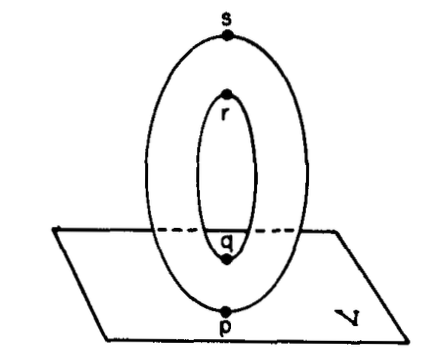
\includegraphics[width=0.4\linewidth]{resources/Diagram1.png}
    \caption{Diagram 1}
    \label{fig:diagram1}
\end{figure}
Let $f: M \rightarrow \mathbb{R}$ be the distance of a point to the plane $V$. 
For a Number $a \in \mathbb{R} $, let $M^a$ be the set of all points $p \in M$, s.th. $f(p) \leq a$.
Then the following are true:
\begin{enumerate}
   \item[(1)] If $a < 0 < f(p)$, then $M^a = \varnothing$
   \item[(2)] If $f(p) < a < f(q)$, then $M^a$ is homeomorphic to a 2-cell.
   \item[(3)] If $f(q) < a < f(r)$, then $M^a$ is homeomorphic tp a cylinder.
   \item[(4)] If $f(q) < a < f(r)$, then $M^a$ is homeomorphic to a compact manifold of genus one with a circle as a boundary.
   \item[(5)] If $f(s) < a$, then $M^a = M$.
\end{enumerate}

To describe how $M^a$ changes as it passes through the points $f(p)$, $f(q)$, $f(r)$, $f(s)$ it is conveniant to consider
homotopy type rather than homeomorphism type. 
\begin{enumerate}[leftmargin=2cm]
   \item[(1) $\rightarrow$ (2)]: In case (1), $M^a$ has the same homotopy type as a point, so this step is the attaching of a 0-cell. 
   \item[(2) $\rightarrow$ (3)]: Is the operation of attaching a 1-cell. 
   \item[(3) $\rightarrow$ (4)]: Again is the operation of attaching a 1-cell. 
   \item[(4) $\rightarrow$ (5)]: Is the action of attaching a 2-cell. 
\end{enumerate}

The definition of attaching a k-cell can be given as follows: \\
Let $S^k = \{x \in \mathbb{R}^{k+1} : \lVert x \rVert = 1\}$ be the $k$-sphere \\
and $D^k = \{ x \in \mathbb{R}^k : \lVert x \rVert \leq 1 \}$ be the $k$-disk.

Let $M$ and $N$ be manifolds, then $N$ is created from $M$ by atteching a k-cell,
if $N$ is of the same homotopy type as a topological space $X$ s.th. there exists 
a pushout square


\end{document}